\chapter*{About}  

\addcontentsline{toc}{chapter}{About}
\thispagestyle{empty}

Hello, I'm M Ahsan Al Mahir, a math olympiad contestant from Bangladesh. I have been with
math olympiads since 2016. And this is my journal of problem solving that I have been
keeping since 2017. 


At the moment of compiling, this journal has \textbf{682} randomly ordered problems,
\textbf{210} theorems and lemmas, and \textbf{174} figures, mostly geometric, drawn in
geogebra and inkscape.

My motivation for keeping the problems I encountered was very significant for me. When I
got serious about math olympiad in 2017, I was really bad at combinatorics. It was a
comletely wild topic, I couldn't seem to find any idea on how to approach any combi
problem whatsoever. So what I decided was to keep a list of general tricks that I would
look through whenever I would try a combinatorial problem. As time went by, that list grew
longer, and so I had to be serious about keeping it organized.

And that's how this journal came to existence. I tried to organize combi problems into the
categories I found were most intuitive, but that wasn't very successful, as the division
between the topics of cominatorics isn't very clear. So expect to find many miscategorized
problems. Also I added anything I found interesting related to olympiad math in this
journal. But as it happens, I didn't follow through with most of those topics, so you
might find a few really fancy beginning of a topic, that never made its way to the second
page.

Also there are a LOT of spelling and grammatical mistakes, as most of the entries I made
here was right after solving (or in most cases, after failing to solve and reading the
solution), I never went back to proofread the comments I left here. So expect a lot of
nonsense talking and typos. Apologies for those :3 

The source files for this journal can be found in my github repository:
\url{https://github.com/AnglyPascal/MO-Problem-Journal}. To compile these files, you will
also need the \texttt{sty} and \texttt{font} files at
\url{https://github.com/AnglyPascal/dotfiles}

\subsection*{How to use this journal}

This journal is divided into chapter/section/subsection manner. Each subsection starts
with a list of useful theorems of lemmas related to that topic, followed by problems and
solutions or hints. Besides the essential theorem and lemmas, I have also added links to
important handouts at the beginning of each section. So check them out if you find the
topics interesting. There are also some boxes titled ``\textbf{Stuck? Try These}'' at the
beginning of the sections, that contain ``rules of thumb'' ideas to keep in mind while
approaching a problem related to that section. 

\thispagestyle{empty}

At the end of the journal, there are four indices: Problems, Theorems, Definitios and
Strategies, that alphabetically list all the items in here. You can use them to quickly
search for a problem or a theorem in this journal.

Most of the problems, theorems and lemmas have links to the AoPS page, Wiki page or
whatever source I learned them from, linked to their titles. Hyperlinks are colored using
\textcolor{urlC}{\textbf{teal green}}. The links between different part of this file are
colored using \textcolor{linkC}{\textbf{teal}}. 

There might be some cases where I missed to link the sources, or couldn't find any
sources. If you notice something like that, please create an issue entry at the github
page, or email me at \url{ahsanalmahir@gmail.com}.

There aren't that many full solutions in this journal, but I listed at least some hints
for most of the problems (though I can't vouch for their usefulness). But you can and
definitely should always visit the AoPS page to look at others solutions.

I intended this journal to be just a list of tricks when I began working on it. Over the
years, this file has grown in size and has become massive. But don't mistake it for a book
or something. Things are all over the place, and not nearly as helpful as an actual
book. But there are interesting things hidden beneath the unorganized texts, and there are
a lot of problems at one place. So it is advised to use it as an extra large problem set
and a resources file rather than a book.

\vspace{2em}

\signature\\
\today


\newpage 
\section*{On ``\texttt{familiarity}'' \\ or, How to avoid ``going down the
\texttt{Math Rabbit Hole}''?}
\thispagestyle{empty}

An excerpt from the
\href{https://math.stackexchange.com/questions/617625/on-familiarity-or-how-to-avoid-going-down-the-math-rabbit-hole}{math.stackexchange
post} of the same title.

Anyone trying to learn mathematics on his/her own has had the experience of ``going down
the Math Rabbit Hole.''

For example, suppose you come across the novel term vector space, and want to learn more
about it. You look up various definitions, and they all refer to something called a field.
So now you're off to learn what a field is, but it's the same story all over again: all
the definitions you find refer to something called a group. Off to learn about what a
group is. Ad infinitum. That's what I'm calling here ``to go down the Math Rabbit Hole.''

Imagine some nice, helpful fellow came along, and made a big graph of every math concept
ever, where each concept is one node and related concepts are connected by edges. Now you
can take a copy of this graph, and color every node green based on whether you ``know''
that concept (unknowns can be grey).

How to define ``know"? In this case, when somebody mentions that concept while talking
about something, do you immediately feel confused and get the urge to look the concept up?
If no, then you know it (funnily enough, you may be deluding yourself into thinking you
know something that you completely misunderstand, and it would be classed as ``knowing''
based on this rule - but that's fine and I'll explain why in a bit). For purposes of
determining whether you ``know'' it, try to assume that the particular thing the person is
talking about isn't some intricate argument that hinges on obscure details of the concept
or bizarre interpretations - it's just mentioned matter-of-factly, as a tangential remark.

When you are studying a topic, you are basically picking one grey node and trying to color
it green. But you may discover that to do this, you must color some adjacent grey nodes
first. So the moment you discover a prerequisite node, you go to color it right away, and
put your original topic on hold. But this node also has prerequisites, so you put it on
hold, and... What you are doing is known as a depth first search. It's natural for it to
feel like a rabbit hole - you are trying to go as deep as possible. The hope is that
sooner or later you will run into a wall of greens, which is when your long, arduous
search will have born fruit, and you will get to feel that unique rush of climbing back up
the stack with your little jewel of recursion terminating return value.

Then you get back to coloring your original node and find out about the other
prerequisite, so now you can do it all over again.

DFS is suited for some applications, but it is bad for others. If your goal is to color
the whole graph (ie. learn all of math), any strategy will have you visit the same number
of nodes, so it doesn't matter as much. But if you are not seriously attempting to learn
everything right now, DFS is not the best choice.

\begin{figure}[H] \centering 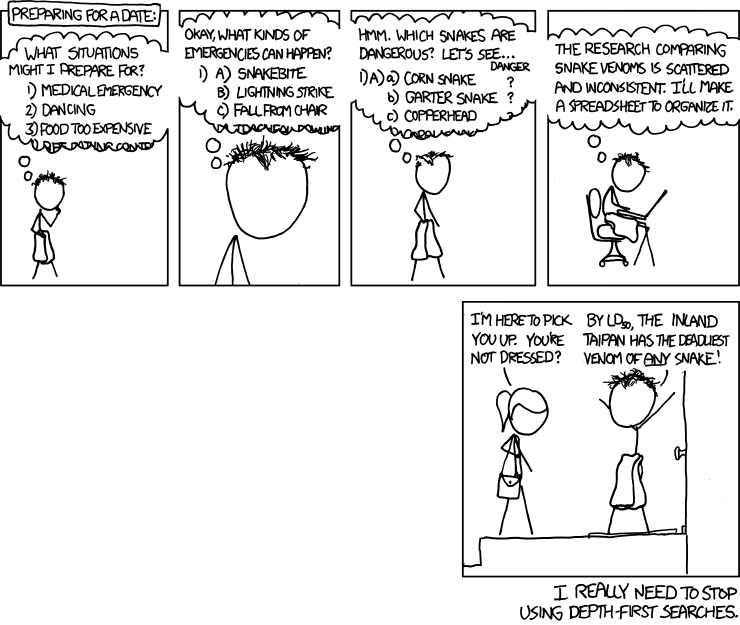
\includegraphics[width=.8\textwidth]{Pics/dfs.png}
\captionsetup{labelformat=empty} \caption{\url{https://xkcd.com/761/}} \end{figure}

So, the solution to your problem is straightforward - use a more appropriate search
algorithm!

\thispagestyle{empty}

Immediately obvious is breadth-first search. This means, when reading an article (or page,
or book chapter), don't rush off to look up every new term as soon as you see it. Circle
it or make a note of it on a separate paper, but force yourself to finish your text even
if its completely incomprehensible to you without knowing the new term. You will now have
a list of prerequisite nodes, and can deal with them in a more organized manner.

Compared to your DFS, this already makes it much easier to avoid straying too far from
your original area of interest. It also has another benefit which is not common in actual
graph problems: Often in math, and in general, understanding is cooperative. If you have a
concept A which has prerequisite concept B and C, you may find that B is very difficult to
understand (it leads down a deep rabbit hole), but only if you don't yet know the very
easy topic C, which if you do, make B very easy to ``get'' because you quickly figure out
the salient and relevant points (or it may be turn out that knowing either B or C is
sufficient to learn A). In this case, you really don't want to have a learning strategy
which will not make sure you do C before B!

BFS not only allows you to exploit cooperativities, but it also allows you to manage your
time better. After your first pass, let's say you ended up with a list of 30 topics you
need to learn first. They won't all be equally hard.  Maybe 10 will take you 5 minutes of
skimming wikipedia to figure out. Maybe another 10 are so simple, that the first Google
Image diagram explains everything. Then there will be 1 or 2 which will take days or even
months of work. You don't want to get tripped up on the big ones while you have the small
ones to take care of. After all, it may turn out that the big topic is not essential, but
the small topic is. If that's the case, you would feel very silly if you tried to tackle
the big topic first! But if the small one proves useless, you haven't really lost much
energy or time.

\thispagestyle{empty}

Once you're doing BFS, you might as well benefit from the other, very nice and clever
twists on it, such as Dijkstra or A*. When you have the list of topics, can you order them
by how promising they seem? Chances are you can, and chances are, your intuition will be
right. Another thing to do - since ultimately, your aim is to link up with some green
nodes, why not try to prioritize topics which seem like they would be getting closer to
things you do know? The beauty of A* is that these heuristics don't even have to be very
correct - even ``wrong'' or ``unrealistic'' heuristics may end up making your search
faster.
